\section{Implementation}
\subsection{Package structure}
Package structure decision was as important task in PokeMongo, we wanted to ensure an high level of readability and maintainability.
Although the classical “root package” which specifies the “domain.company.projet”, in our case “it.unipi.dii.lsmsd.pokemongo”, all the packages are structured \textit{by layers}. In this way, we decided to name the packages according to they function architecturally rather than their identity according to the business domain. Here the structure: 

\begin{figure}[H]
	\centering
	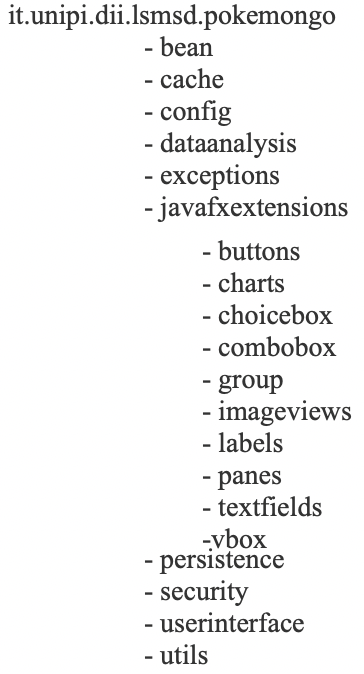
\includegraphics[width= 0.3\textwidth]{img/package_structure.png}
	\caption{Package Structure}
\end{figure}

We tried to maintain the name of the packages as simple as possible, and in a way they are all easy to read and to understand.
We also followed the convention of having the first character in the package names in lower case, in order to avoid conflicts with class or interface names.

\subsubsection{Package Analysis: Bean}
The “bean” package contains few classes that are used as beans while the application runs.

\begin{figure}[H]
	\centering
	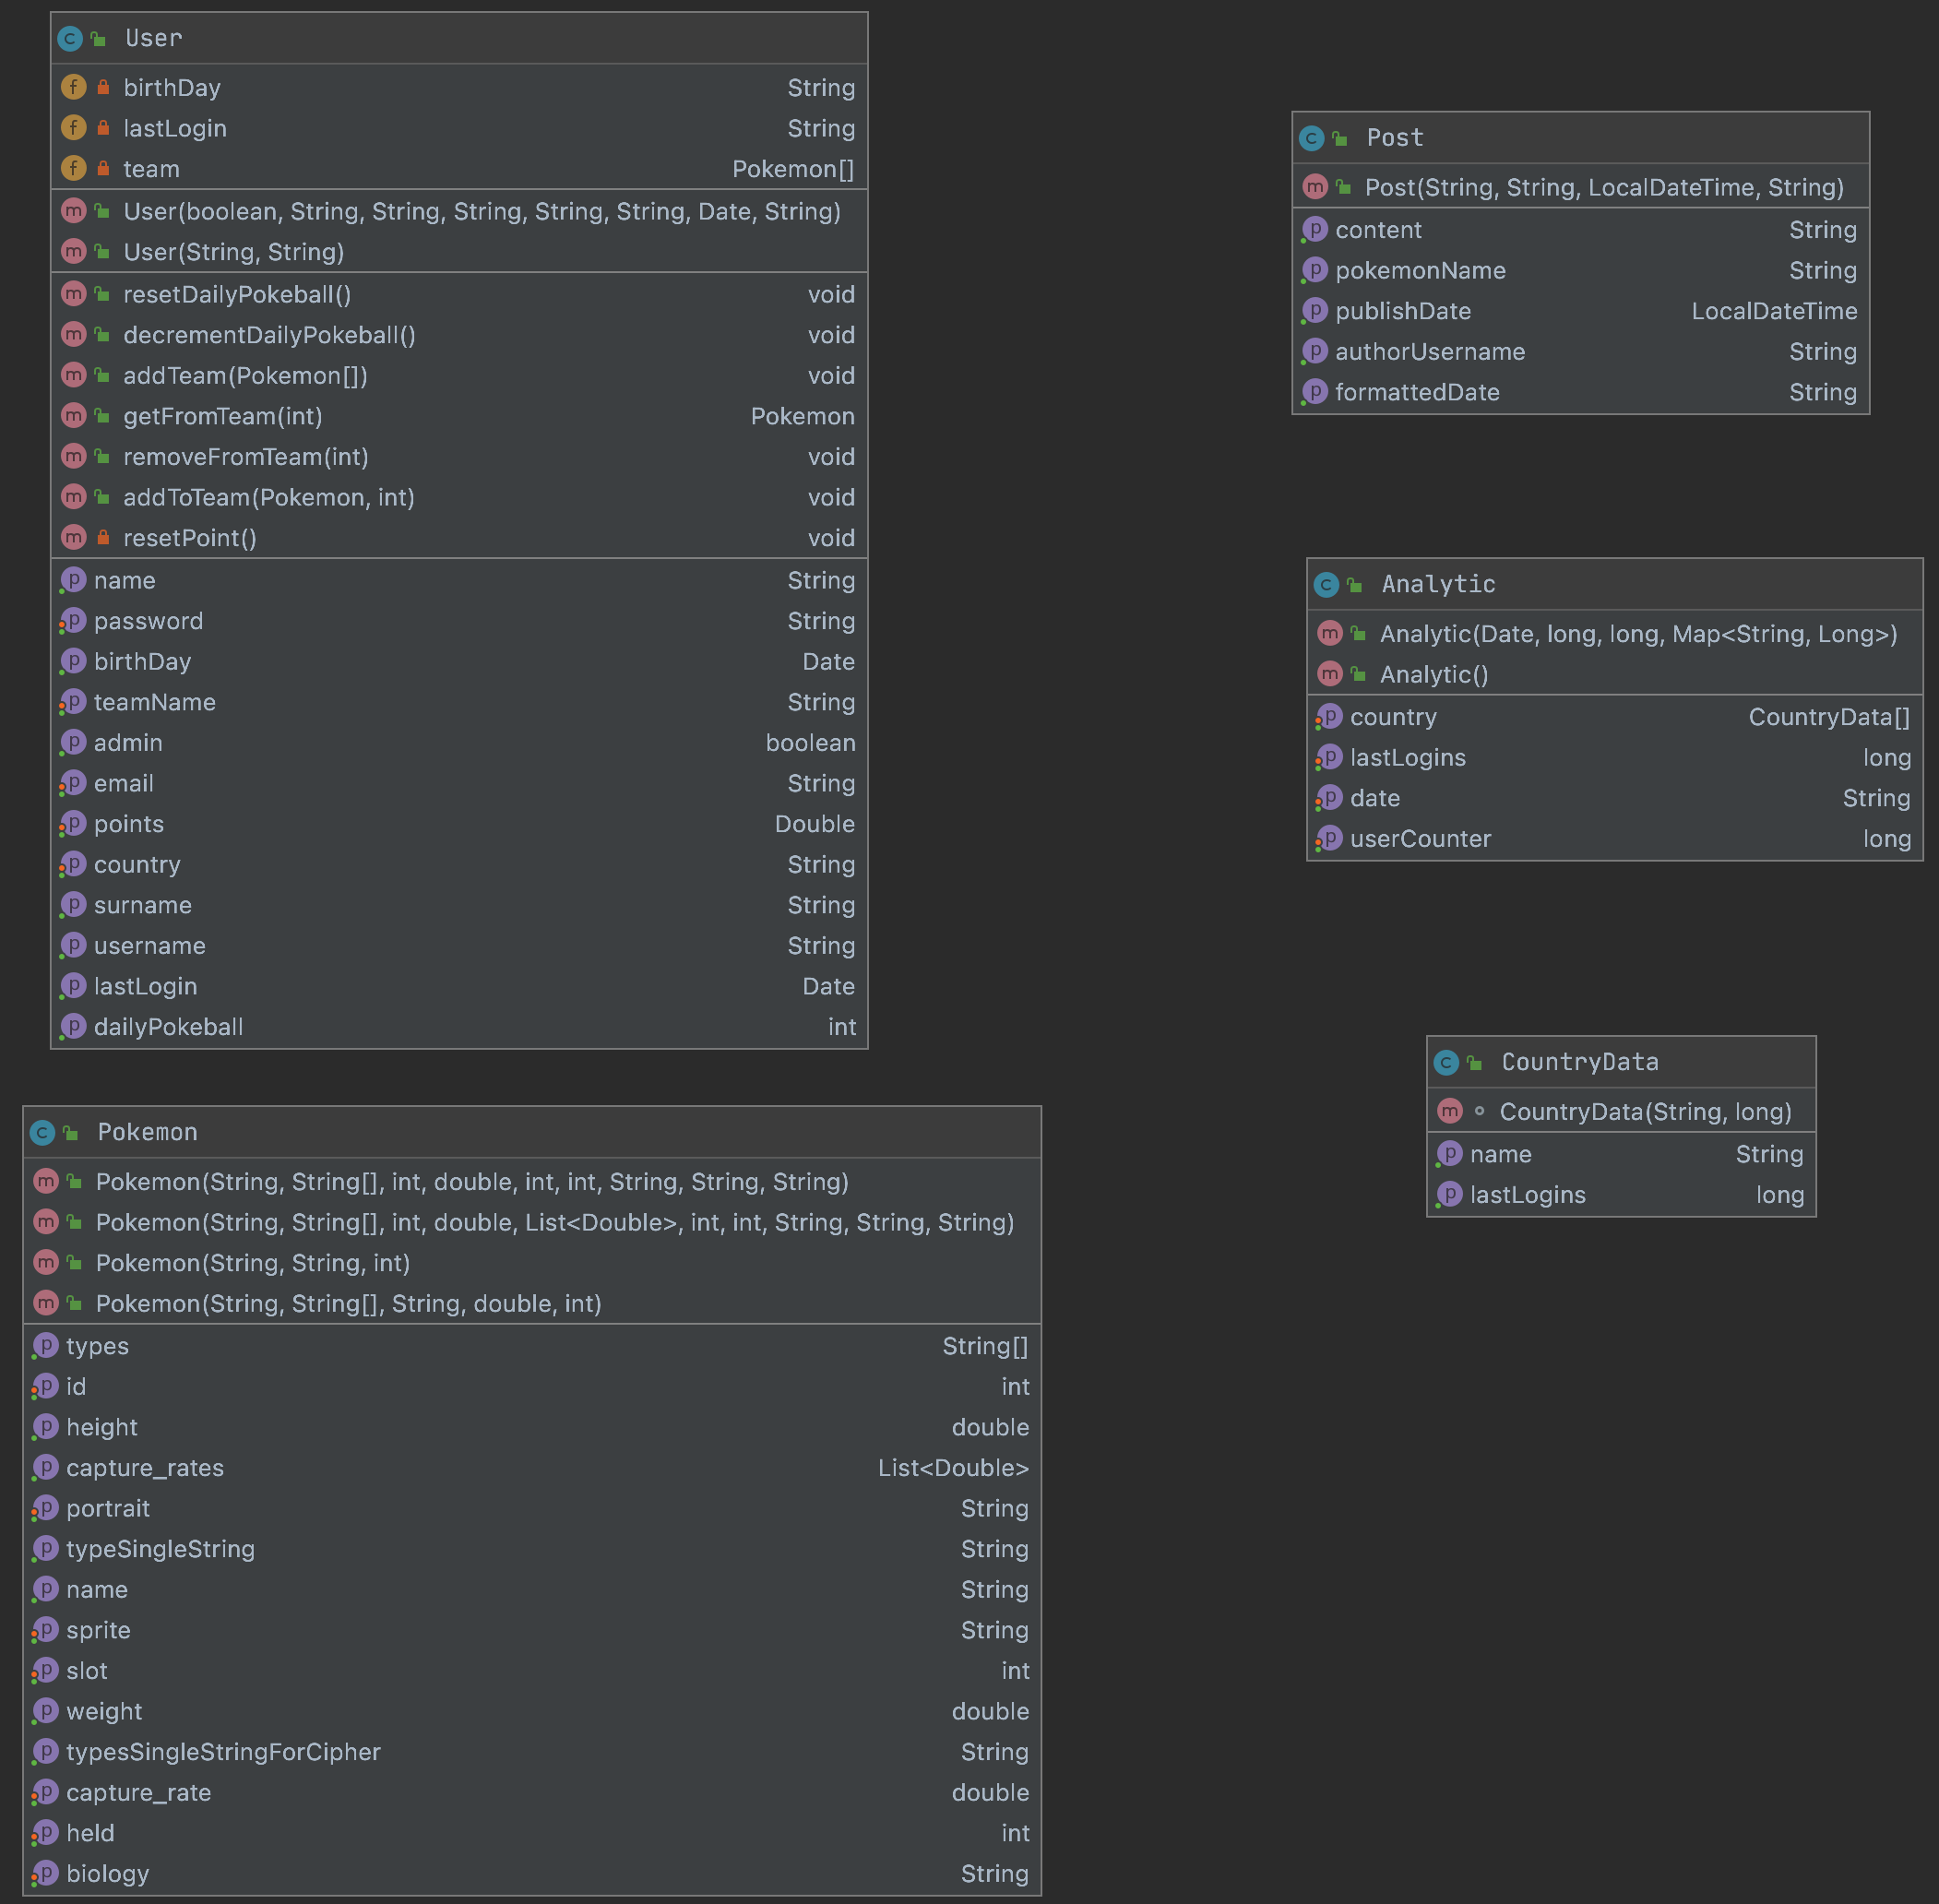
\includegraphics[width=0.9\textwidth]{img/bean_package.png}
	\caption{Bean Package Class Structure}
\end{figure}

\begin{center}
	\begin{tabular}{| m{9em} | m{22em} |} 
		\hline
		\textbf{Class Name} & \textbf{Short Description} \\ [0.5ex] 
		\hline
		User & The User class is used for instantiating object that refers to a specific user\\ 
		\hline
		Pokemon & The Pokemon class is used for instantiating object that refers to a specific Pokemon\\
		\hline
		Post & The Post class is used for instantiating object that refers to a specific Post. Responses (aka subPosts) are considered post also.\\
		\hline
		Analytic & This class is used for containing the information regarding a particular day.\\
		\hline
		CountryData & Used in the Analytic bean, it contains the information regarding a single country and the analytic strictly associated to it.\\
		\hline
	\end{tabular}
\end{center}

\subsubsection{Package Analysis: Cache}
The cache package contains classes that are helpful for caching images, we will talk about that in chapter 4.3.2. Despite what written above, this is one of the few packages that has a feature logic structure inside. We maintain in this package not only the classes/interface that handle the caching functionality, but also a javafx class extension which is PokemonImage. This class is strictly connected to the caching systems, because it contains the image we want to cache. We decided to use this approach to have a cleaner look and an easier maintainability for the caching systems. 
\begin{figure}[H]
	\centering
	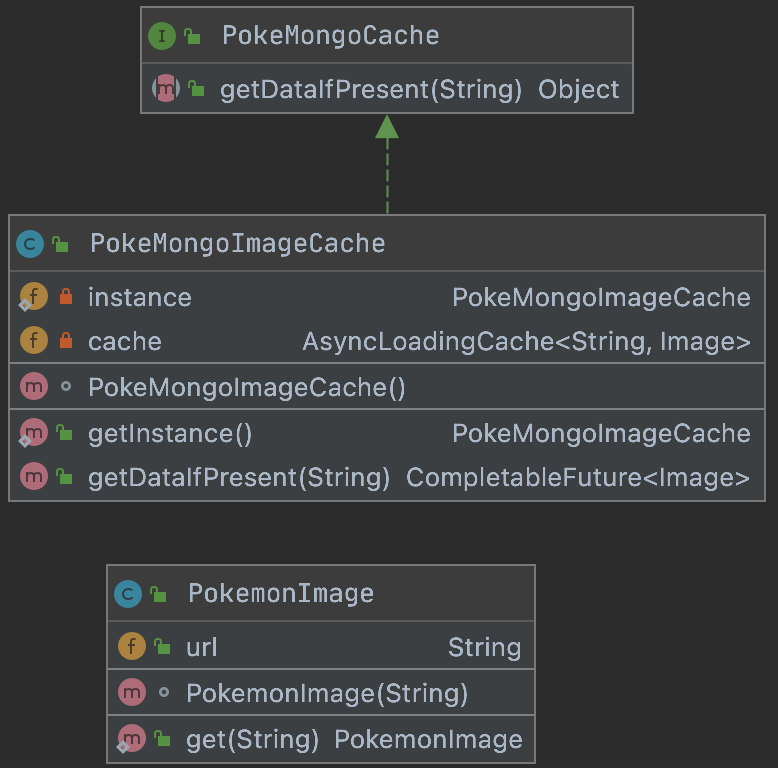
\includegraphics[width=0.4\textwidth]{img/cache_package.png}
	\caption{Cache Package Class Structure}
\end{figure}

\begin{center}
	\begin{tabular}{| m{14em} | m{19em} |} 
		\hline
		\textbf{Class Name} & \textbf{Short Description} \\ [0.5ex] 
		\hline
		PokeMongoCache & Simply an interface.\\ 
		\hline
		PokeMongoImageCache & The implementation of the interface described.\\ 
		\hline
		PokemonImage & An Image (javaFX) extension that will contains the image we want to show to the user in the GUI.\\ 
		\hline
	\end{tabular}
\end{center}

\subsubsection{Package Analysis: dataAnalysis}
This package is used for instantiating factory structures about the data analysis we made in the project. Every factory is dependent of an interface. 

\begin{figure}[H]
	\centering
	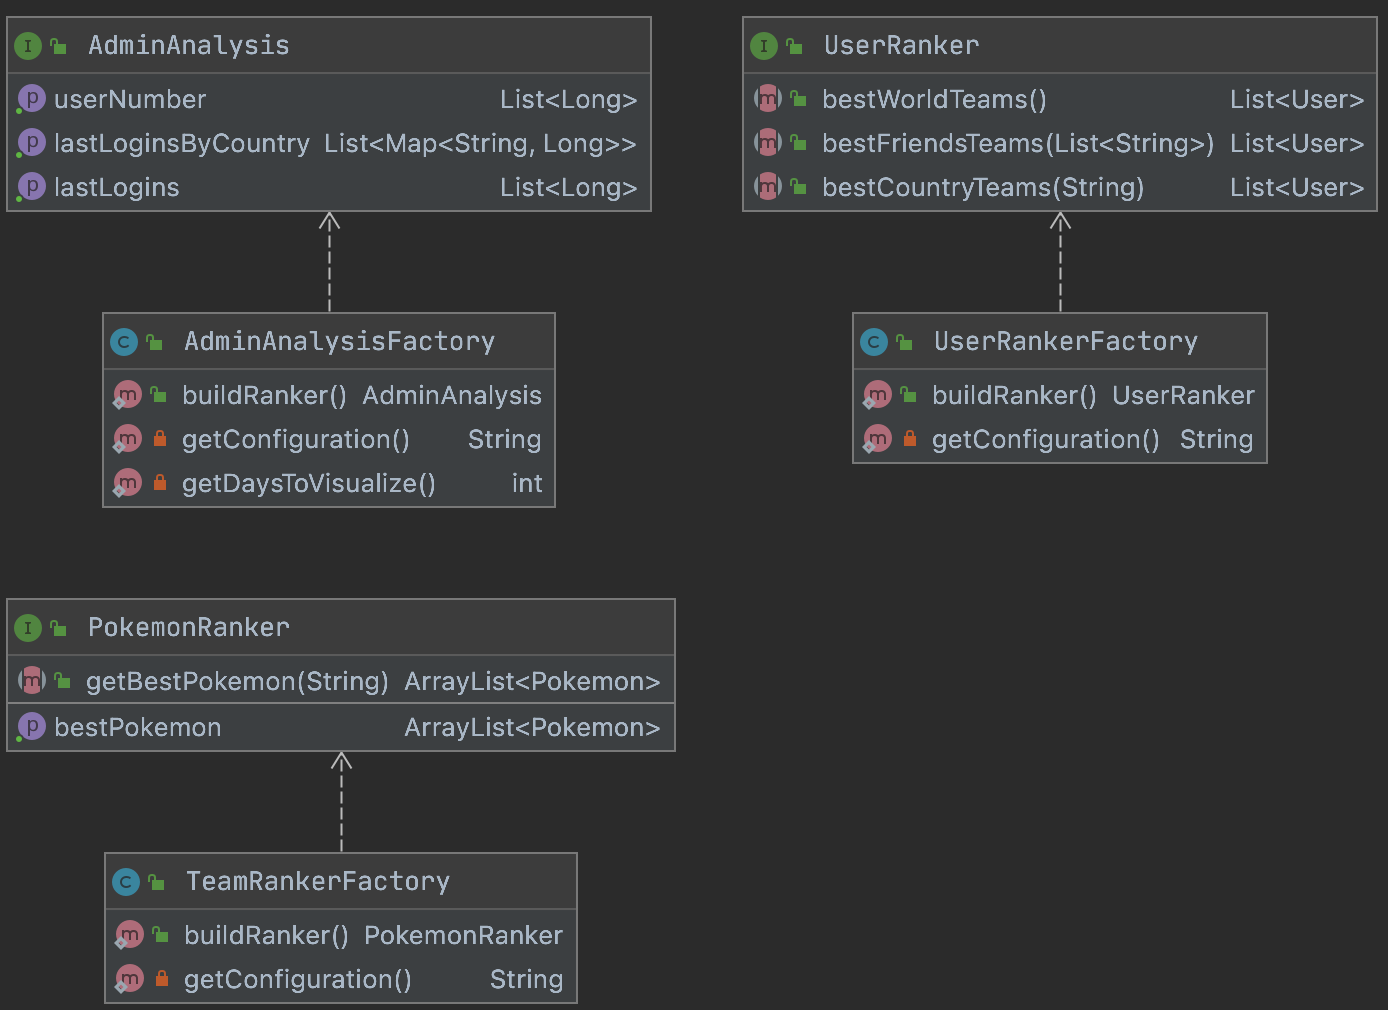
\includegraphics[width=0.7\textwidth]{img/dataAnalysis_package.png}
	\caption{dataAnalysis Package Class Structure}
\end{figure}

\begin{center}
	\begin{tabular}{| m{14em} | m{19em} |} 
		\hline
		\textbf{Class Name} & \textbf{Short Description} \\ [0.5ex] 
		\hline
		AdminAnalytics &Simply an interface for the analytics related to the admin user\\ 
		\hline
		AdminAnalysisFactory & Has a static method that returns a specific implementation of the interface AdminAnalytics\\ 
		\hline
		UserRanker & Simply an interface for the analytics for user ranking.\\ 
		\hline
		UserRankerFactory & Has a static method that returns a specific implementation of the interface UserRanker\\ 
		\hline
		PokemonRanker & Simply an interface for the analytics for pokemon ranking\\ 
		\hline
		PokemonRankerFactory & Has a static method that returns a specific implementation of the interface PokemonRanker\\
		\hline
	\end{tabular}
\end{center}

\subsubsection{Package Analysis: exceptions}
This package contains classes that extend the class Exception of Java. 
\begin{figure}[H]
	\centering
	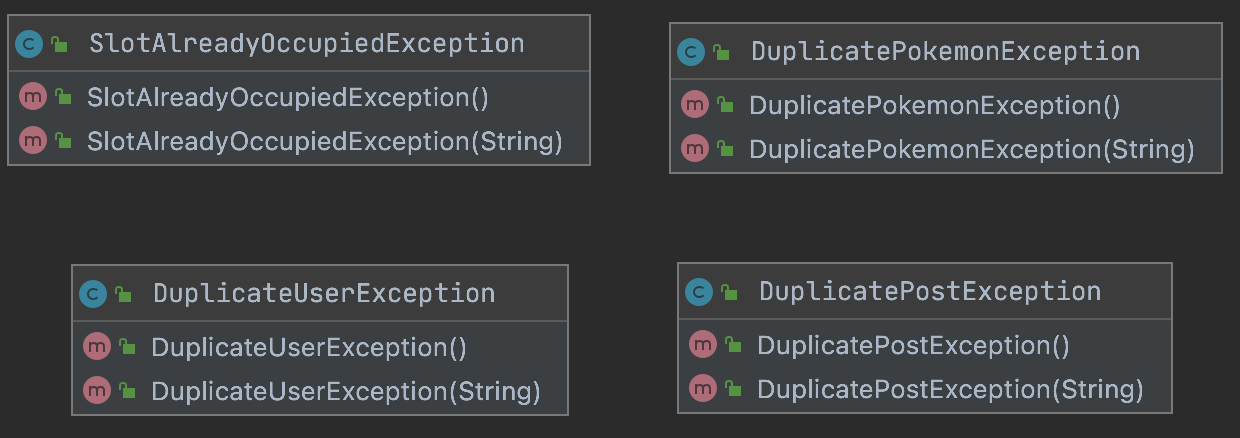
\includegraphics[width=0.7\textwidth]{img/exceptions_package.png}
	\caption{Exceptions Package Class Structure}
\end{figure}
\begin{center}
	\begin{tabular}{| m{14em} | m{19em} |} 
		\hline
		\textbf{Class Name} & \textbf{Short Description} \\ [0.5ex] 
		\hline
		SlotAlreadyOccupiedException &Exception thrown when a user try to catch a Pokemon and he has the slot he want to use already occupied by one other Pokemon\\ 
		\hline
		DuplicatePokemonException & Exception thrown when an admin try to insert a Pokemon that is already present\\ 
		\hline
		DuplicateUserException & Exception thrown when an anonymous user try to create a register user, but the username he writes is already taken.\\ 
		\hline
		DuplicatePostException & Exception thrown if an identical Post is created\\ 
		\hline
	\end{tabular}
\end{center}
\subsubsection{Package Analysis: javafxextensions}
In this package are present 11 sub-packages, any of them related to a specific extension of a JavaFX Node.
\subparagraph{javafxextensions: buttons}
Here are present all the classes that extend Button from JavaFX
\begin{figure}[H]
	\centering
	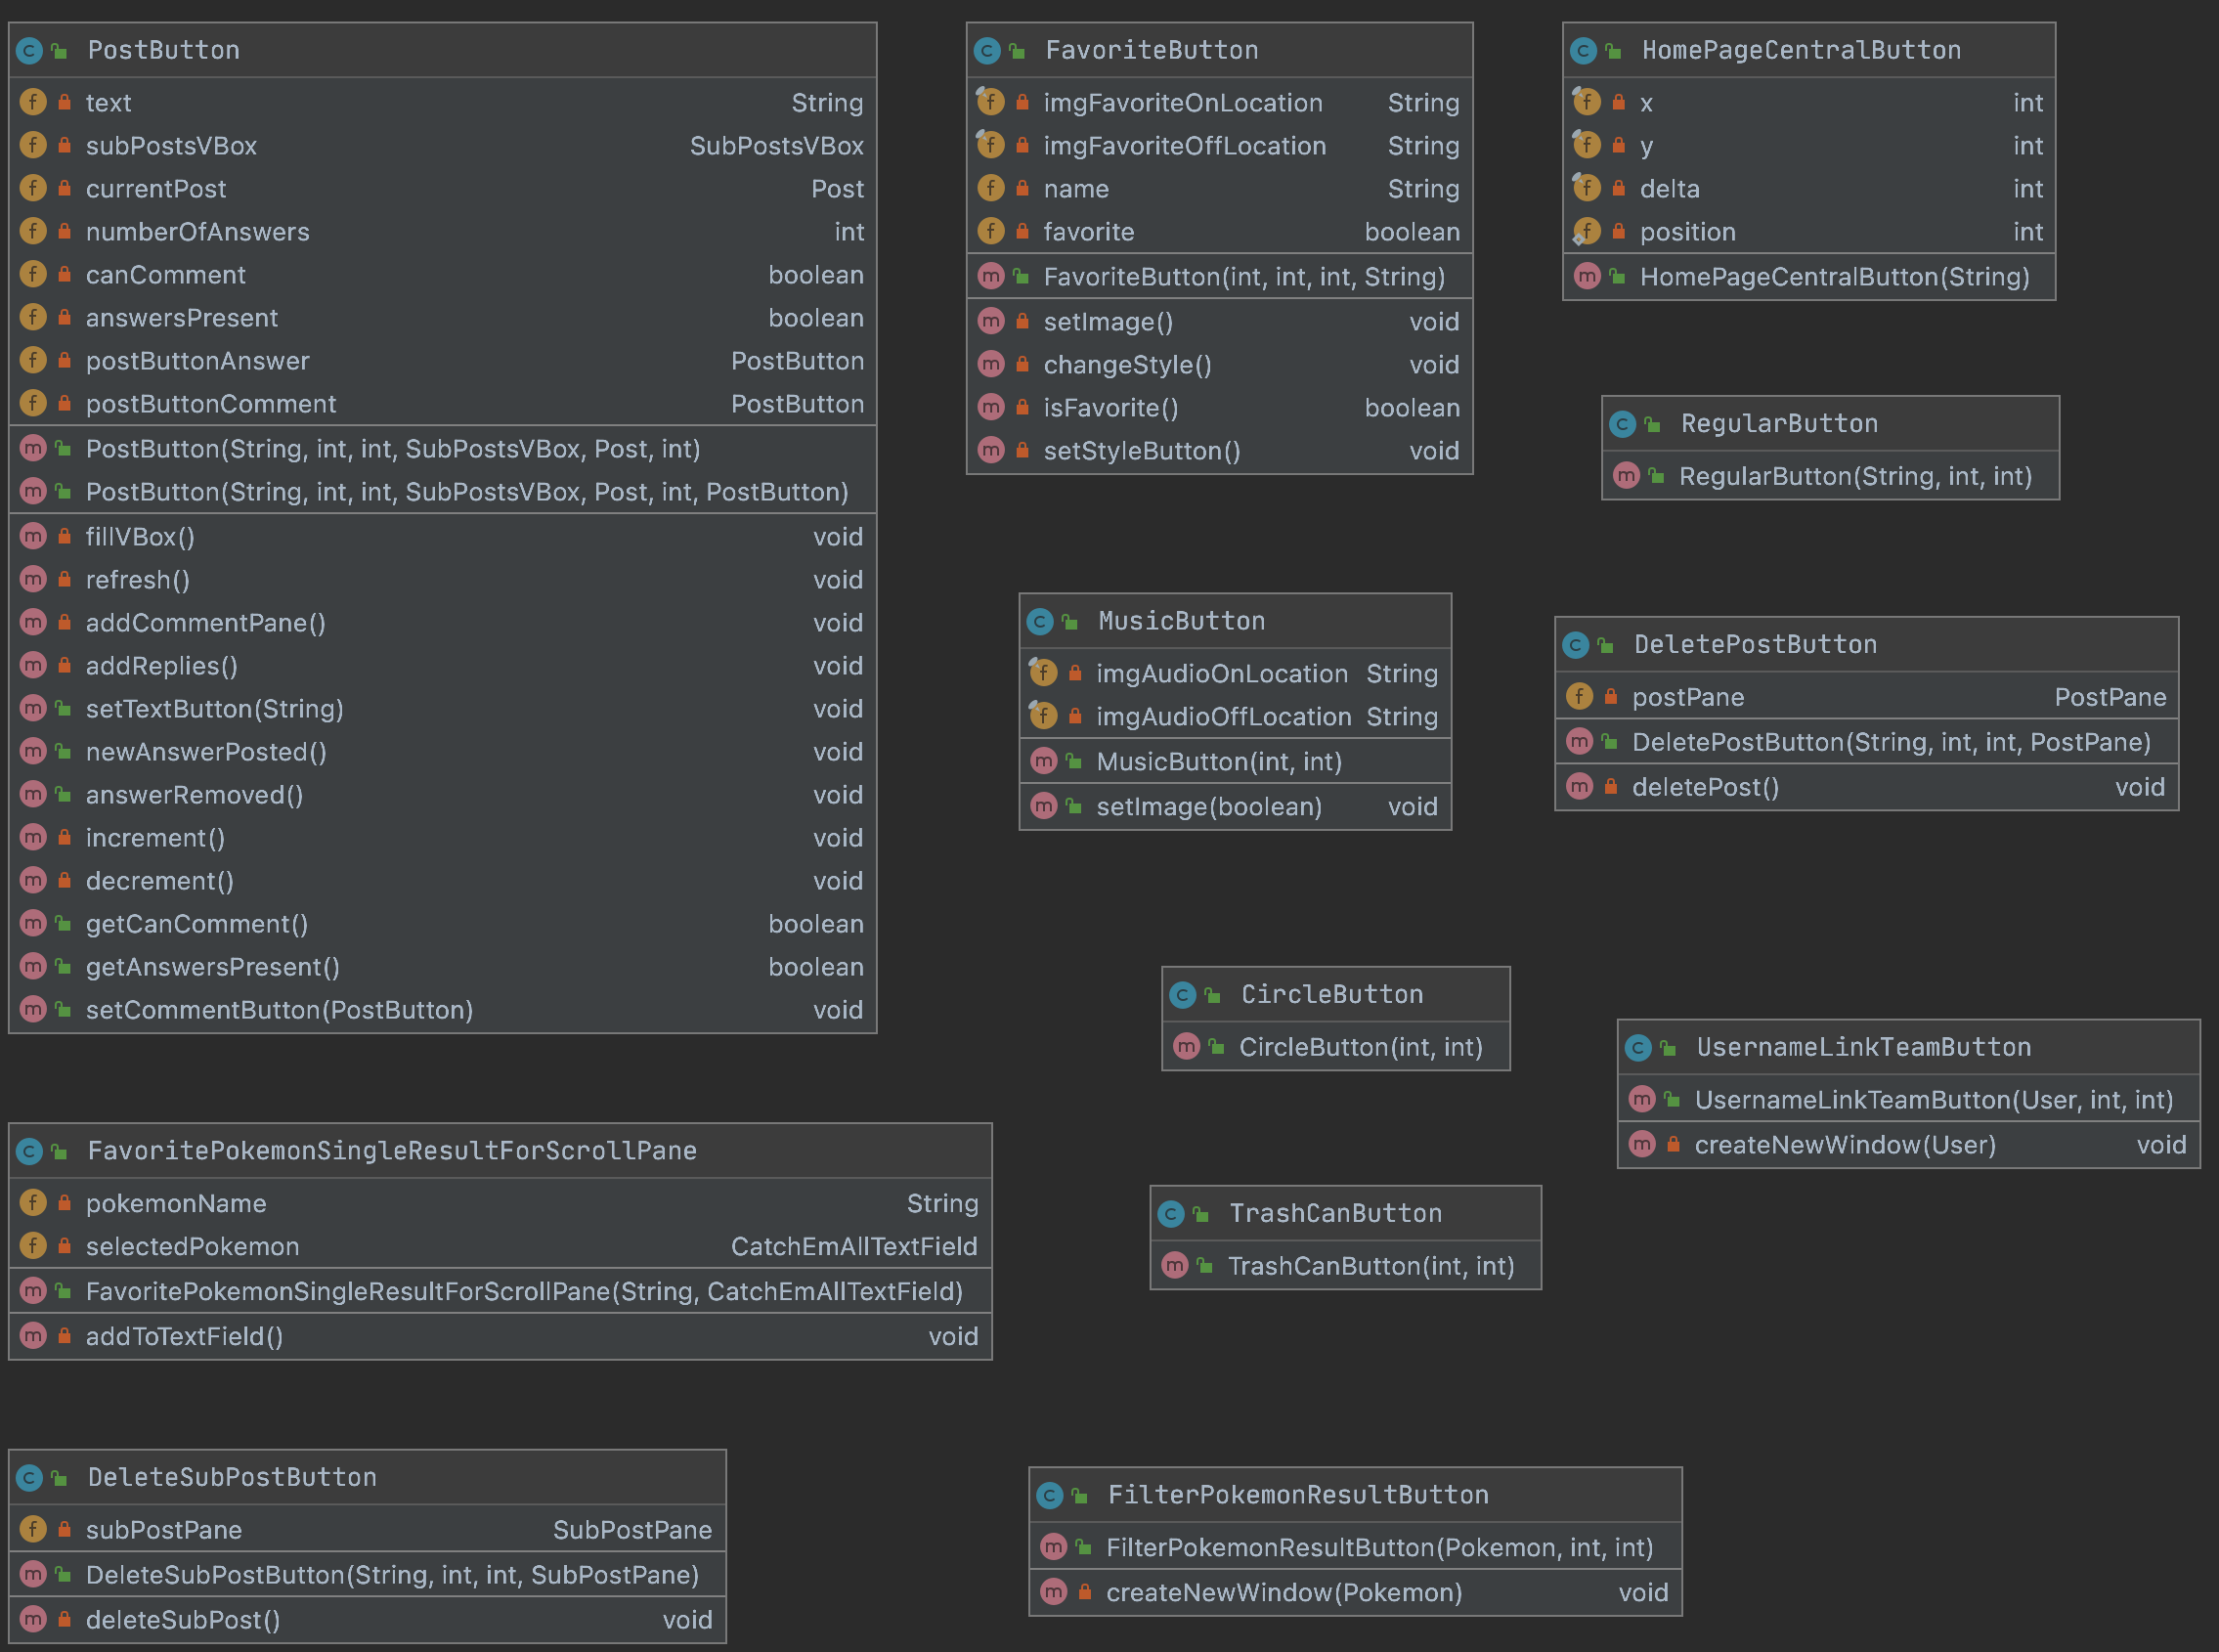
\includegraphics[width=0.7\textwidth]{img/javafx_buttons_package.png}
	\caption{javafxExtension/buttons Package Class Structure}
\end{figure}
\begin{center}
	\begin{longtable}{| m{14em} | m{19em} |} 
		\hline
		\textbf{Class Name} & \textbf{Short Description} \\ [0.5ex] 
		\hline
		HomePageCentralButton & Specific button for the HomePage.\\ 
		\hline
		MusicButton & Button for turning the music on/off\\ 
		\hline
		RegularButton & For creating buttons like “BACK”, “SUBMIT”, etc…\\ 
		\hline
		TrashButton & Button for eliminating a Pokemon in the Team\\ 
		\hline
		CircleButton & Helpful for creating button with a circular shape\\ 
		\hline
		PostButton & Specific button for submitting a comment in the post section of a Pokemon\\
		\hline
		DeletePostButton & Button for deleting a SubPost (aka response)\\
		\hline
		FilterPokemonResultButton & Specific button for displaying the name of a Pokemon in a query result. At the click it creates a new Stage with the information about the Pokemon (check PokemonWindowGroup).\\
		\hline
		FavoritePokemonSingleResultFor ScrollPane & This button is used for showing the name of the Pokemon than are Favourite. Clicking on it will be a shortcut for capturing the Pokemon the button says about.\\
		\hline
		UsernameLinkTeamButton & Specific button for displaying the username of a User in a query result. At the click it creates a new Stage with the team of the User (check TeamUserWindowGroup).\\
		\hline
	\end{longtable}
\end{center}
\subparagraph{javafxextensions: charts}
It contains a class that extends LineChart from JavaFX.
\begin{figure}[H]
	\centering
	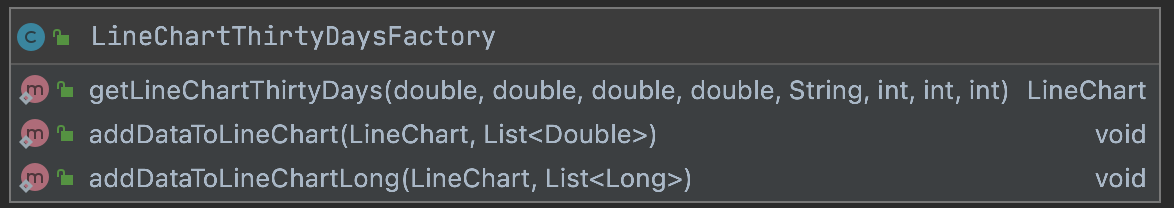
\includegraphics[width=0.7\textwidth]{img/javafx_charts_package.png}
	\caption{javafxExtensions/charts Package Class Structure}
\end{figure}
\begin{center}
	\begin{tabular}{| m{14em} | m{19em} |} 
		\hline
		\textbf{Class Name} & \textbf{Short Description} \\ [0.5ex] 
		\hline
		LineChartThirtyDaysFactory & The class helps for the creation of different Line Charts, which can have different meanings (e.g. number of logins, number of users, …)  This is used for every plot in the application\\ 
		\hline
	\end{tabular}
\end{center}
\subparagraph{javafxextensions: choicebox}
It contains a class that extends LineChart from JavaFX.
\begin{figure}[H]
	\centering
	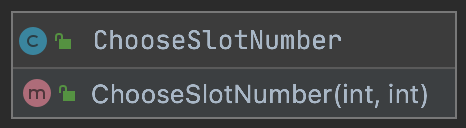
\includegraphics[width=0.5\textwidth]{img/javafx_choicebox_package.png}
	\caption{javafxExtensions/choicebox Package Class Structure}
\end{figure}
\begin{center}
	\begin{tabular}{| m{14em} | m{19em} |} 
		\hline
		\textbf{Class Name} & \textbf{Short Description} \\ [0.5ex] 
		\hline
		ChooseSlotNumber & Choice box that lets the user to select the slot for saving the Pokemon in captured\\ 
		\hline
	\end{tabular}
\end{center}
\subparagraph{javafxextensions: combobox}
A ComboBox can be seen as a ChoiceBox, the user select the elements in it in the same way.
\begin{figure}[H]
	\centering
	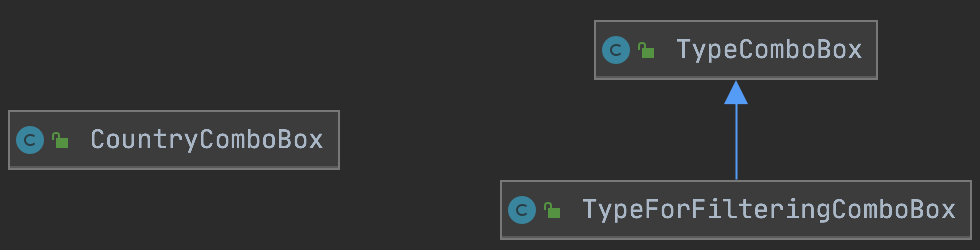
\includegraphics[width=0.8\textwidth]{img/javafx_combobox_package.png}
	\caption{javafxExtensions/combobox Package Class Structure}
\end{figure}
\begin{center}
	\begin{tabular}{| m{14em} | m{19em} |} 
		\hline
		\textbf{Class Name} & \textbf{Short Description} \\ [0.5ex] 
		\hline
		CountryComboBox & Let the user to select the country\\ 
		\hline
		TypeComboBox & General ComboBox for choosing the type of a pokemon\\ 
		\hline
		TypeForFilteringComboBox & Specific TypeComboBox for the filtering Pane.\\ 
		\hline
	\end{tabular}
\end{center}

\subparagraph{javafxextensions: group}
The group extensions are used for creating new windows with particular information regarding something. 
\begin{figure}[H]
	\centering
	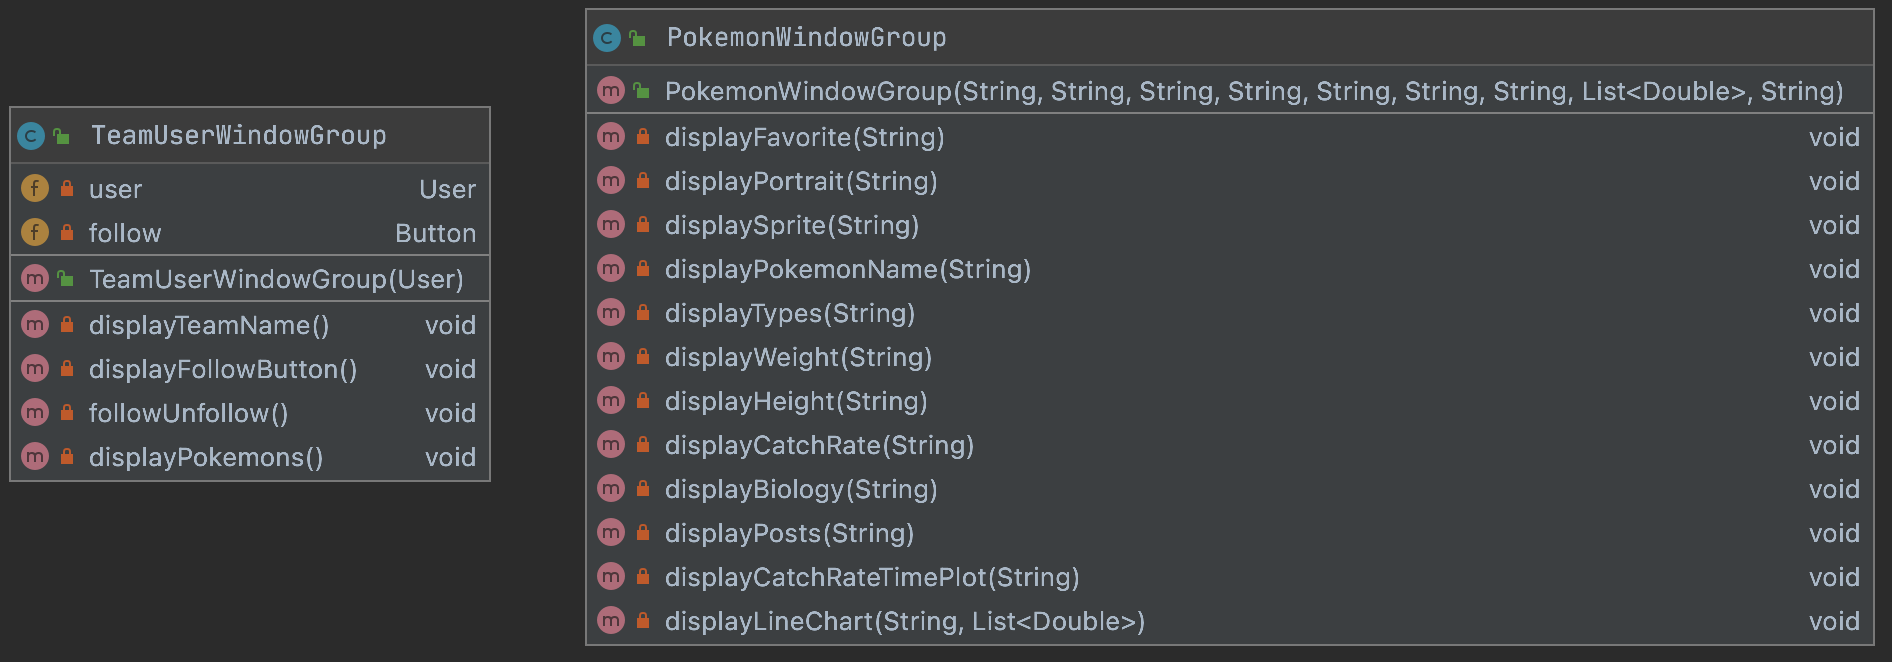
\includegraphics[width=0.8\textwidth]{img/javafx_group_package.png}
	\caption{javafxExtensions/group Package Class Structure}
\end{figure}
\begin{center}
	\begin{tabular}{| m{14em} | m{19em} |} 
		\hline
		\textbf{Class Name} & \textbf{Short Description} \\ [0.5ex] 
		\hline
		TeamUserWindowGroup & Instantiates all the Node that are needed for creating the window which display the team of a specific user\\ 
		\hline
		PokemonWindowGroup & Instantiates all the Node that are needed for creating the window which display the information of a specific Pokemon along with the posts related to it\\ 
		\hline
	\end{tabular}
\end{center}
\subparagraph{javafxextensions: imageviews}
Extensions of ImageView
\begin{figure}[H]
	\centering
	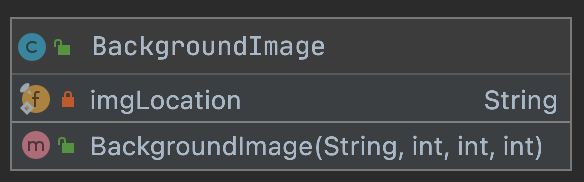
\includegraphics[width=0.5\textwidth]{img/javafx_imageviews_package.png}
	\caption{javafxExtensions/imageviews Package Class Structure}
\end{figure}
\begin{center}
	\begin{tabular}{| m{14em} | m{19em} |} 
		\hline
		\textbf{Class Name} & \textbf{Short Description} \\ [0.5ex] 
		\hline
		BackgroundImage & Helpful for adding image in the background.\\ 
		\hline
	\end{tabular}
\end{center}

\subparagraph{javafxextensions: labels}
This package contains different types of labels useful for different situations.
\begin{figure}[H]
	\centering
	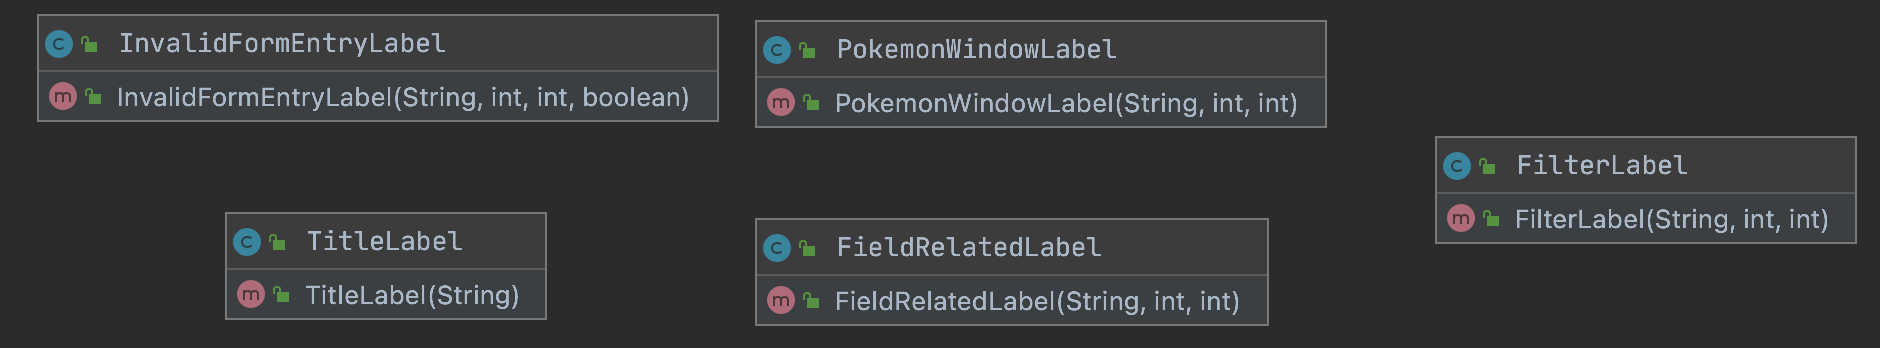
\includegraphics[width=0.8\textwidth]{img/javafx_labels_package.png}
	\caption{javafxExtensions/labels Package Class Structure}
\end{figure}
\begin{center}
	\begin{tabular}{| m{14em} | m{19em} |} 
		\hline
		\textbf{Class Name} & \textbf{Short Description} \\ [0.5ex] 
		\hline
		InvalidFormEntryLabel & Used when an error occurs at the filling of an entry in a form.\\ 
		\hline
		PokemonWindowLabel & A specific Label that is used in the Stage created with the information of the a specific Pokemon\\ 
		\hline
		TitleLabel & Used for creating title in a prefix position.\\ 
		\hline
		FieldRelatedLabel & Used to indicate what a TextField is related to\\ 
		\hline
		FieldLabel & Used for the labels in the filter Pane\\ 
		\hline
	\end{tabular}
\end{center}
\subparagraph{javafxextensions: panes}
The Panes are the most important JavaFX extension we made in the project. The Panes help the system to be more modular. Modularity by the Panes is archived by dividing every complex components of the GUI in sub components that can be used and modified as stand alone (this gives us also an high level of maintainability). Only one type of Pane is standing separated by the others, inside the addPane package contained in the pane package, this because this pane is strictly connected to an enum that is present in that same folder (we just want to divide this particular enum, to the rest of the panes that, in fact, do not interact with it). 
\begin{figure}[H]
	\centering
	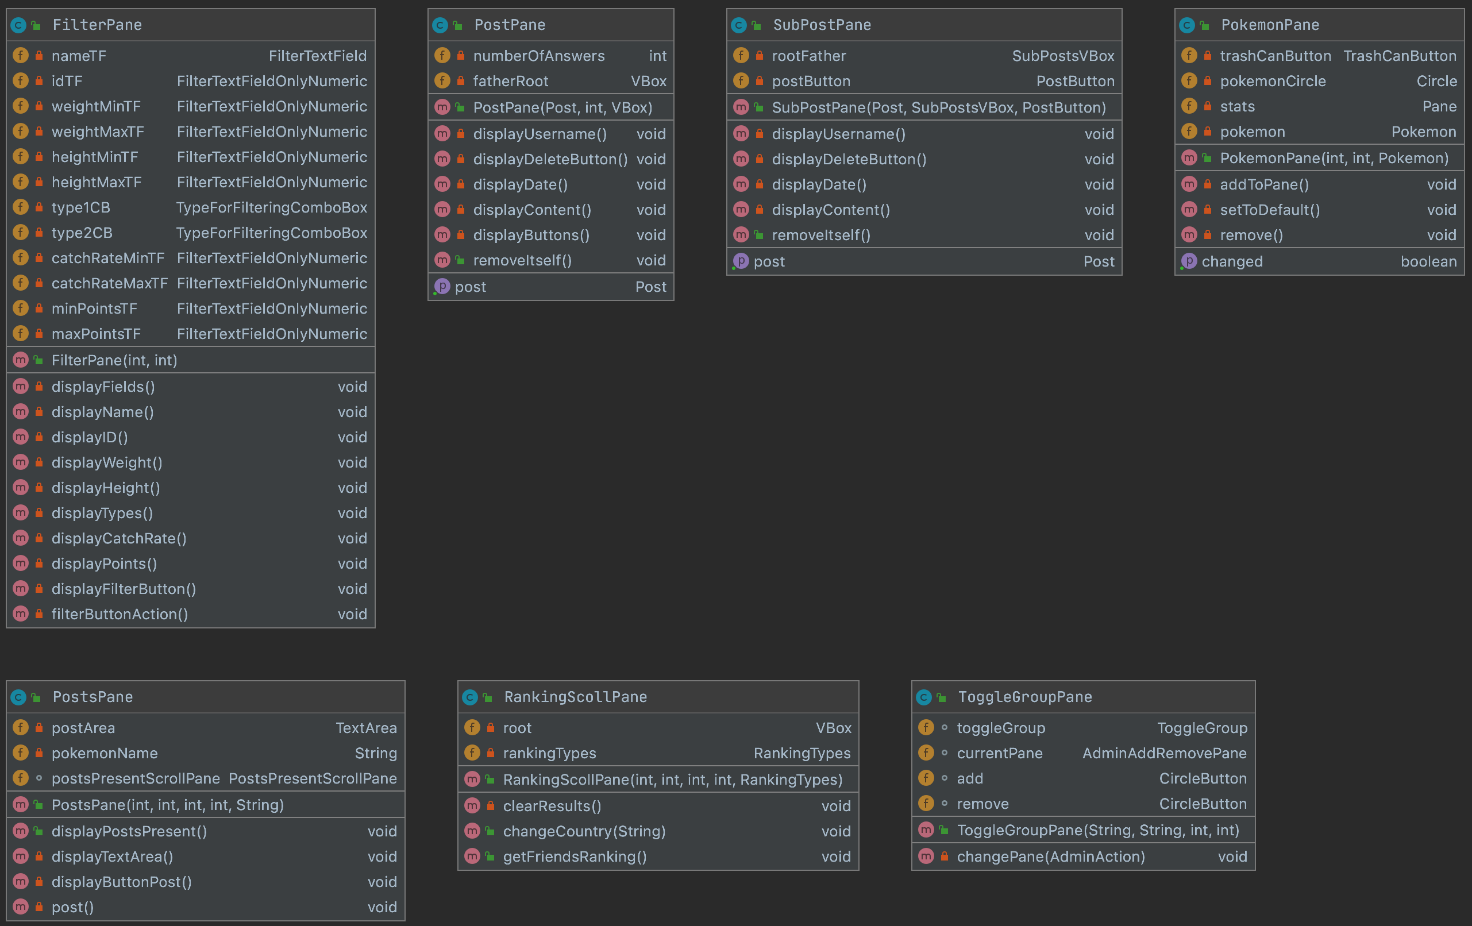
\includegraphics[width=\textwidth]{img/javafx_panes_package.png}
\end{figure}
\begin{figure}[H]
	\centering
	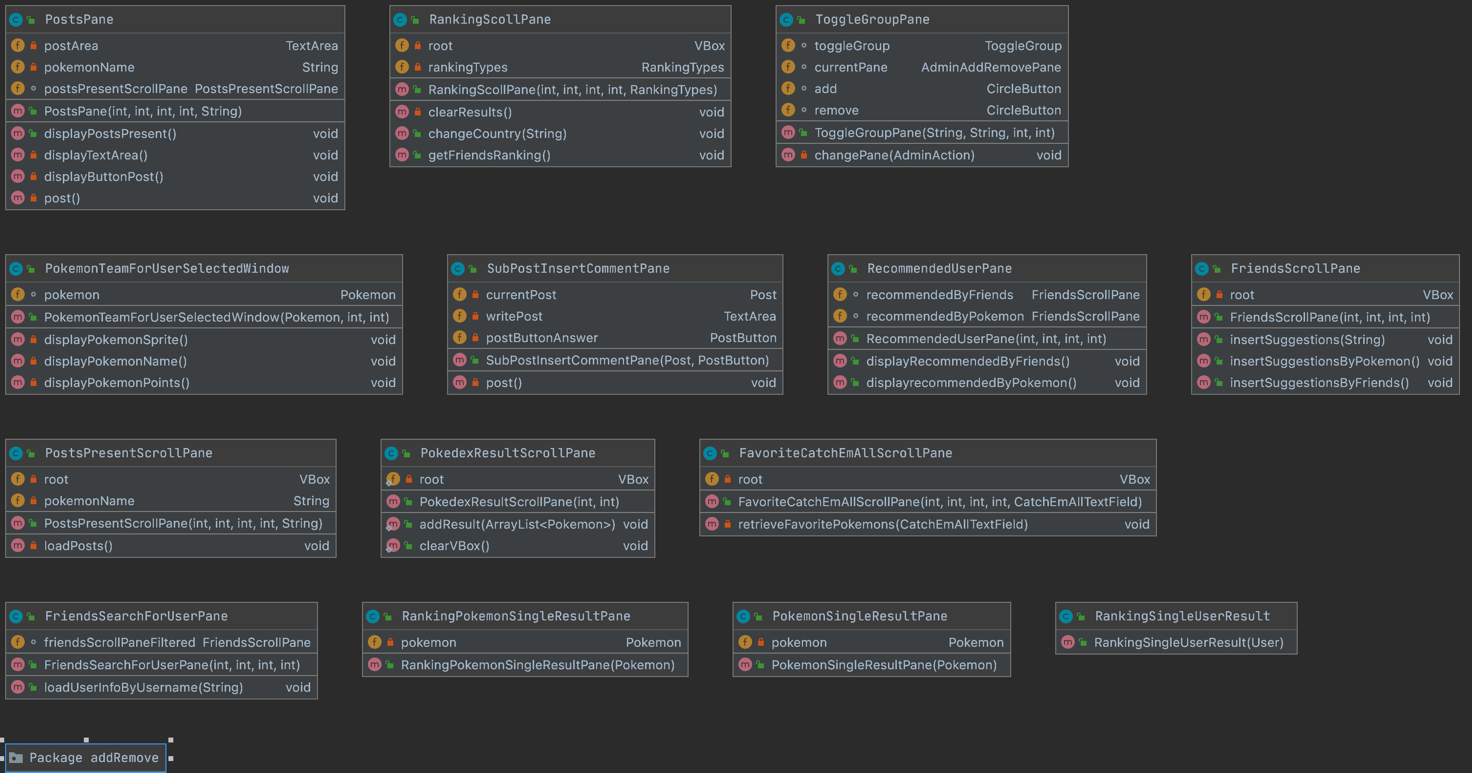
\includegraphics[width=\textwidth]{img/javafx_panes_package2.png}
	\caption{javafxExtensions/panes Package Class Structure}
\end{figure}
\begin{center}
	\begin{longtable}{| m{14em} | m{19em} |} 
		\hline
		\textbf{Class Name} & \textbf{Short Description} \\ [0.5ex] 
		\hline
		RankingScrollPane & Pane that can be scrolled. It contains other panes that are specific for something (e.g. a user, a Pokemon).\\ 
		\hline
		ToggleGroupPane & Specific pane for creating a toggle group.n\\ 
		\hline
		PokemonTeamForUserSelected Window & Specific pane for showing a single Pokemon in the other user window.\\ 
		\hline
		SubPostInsertCommentPane & Specific pane that is used to create the Nodes for a response to a Post. The need of that comes by the fact the TextArea and the button in it should be horizontal to each other (impossible in the VBox this Pane it’s used).\\ 
		\hline
		RecommendedUserPane & Specific Pane for the recommended section in the Friends page.\\ 
		\hline
		FriendsScrollPane & Specific ScrollPane to visualize friends users (an even the one recommended).\\ 
		\hline
		PostsPresentScrollPane & Specific ScrollPane to visualize a limited number of Posts.\\ 
		\hline
		PokedexResultScrollPane & Specific ScrollPane to visualize the result of a filtering operation.\\ 
		\hline
		FavoriteCatchEmAllScrollPane & Specific ScrollPane to visualize the Pokemon set as favorite\\ 
		\hline
		FriendsSearchForUserPane & Specific pane for searching an user (Friends scene)\\ 
		\hline
		RankingPokemonSingleResult PaneSpecific & Specific pane to be inserted in a ScrollPane extension. It gives some information about the Pokemon (used in the Ranking)\\ 
		\hline
		PokemonSingleResultPane & Specific pane to be inserted in a ScrollPane extension. It gives some information about the Pokemon (used in the Pokedex)\\
		\hline
		RankingSingleUserResult & Specific pane to be inserted in a ScrollPane extension. It gives some information about the Pokemon (used in the Ranking)\\
		\hline
	\end{longtable}
\end{center}

The addRemove package is characterized of these classes:
\begin{figure}[H]
	\centering
	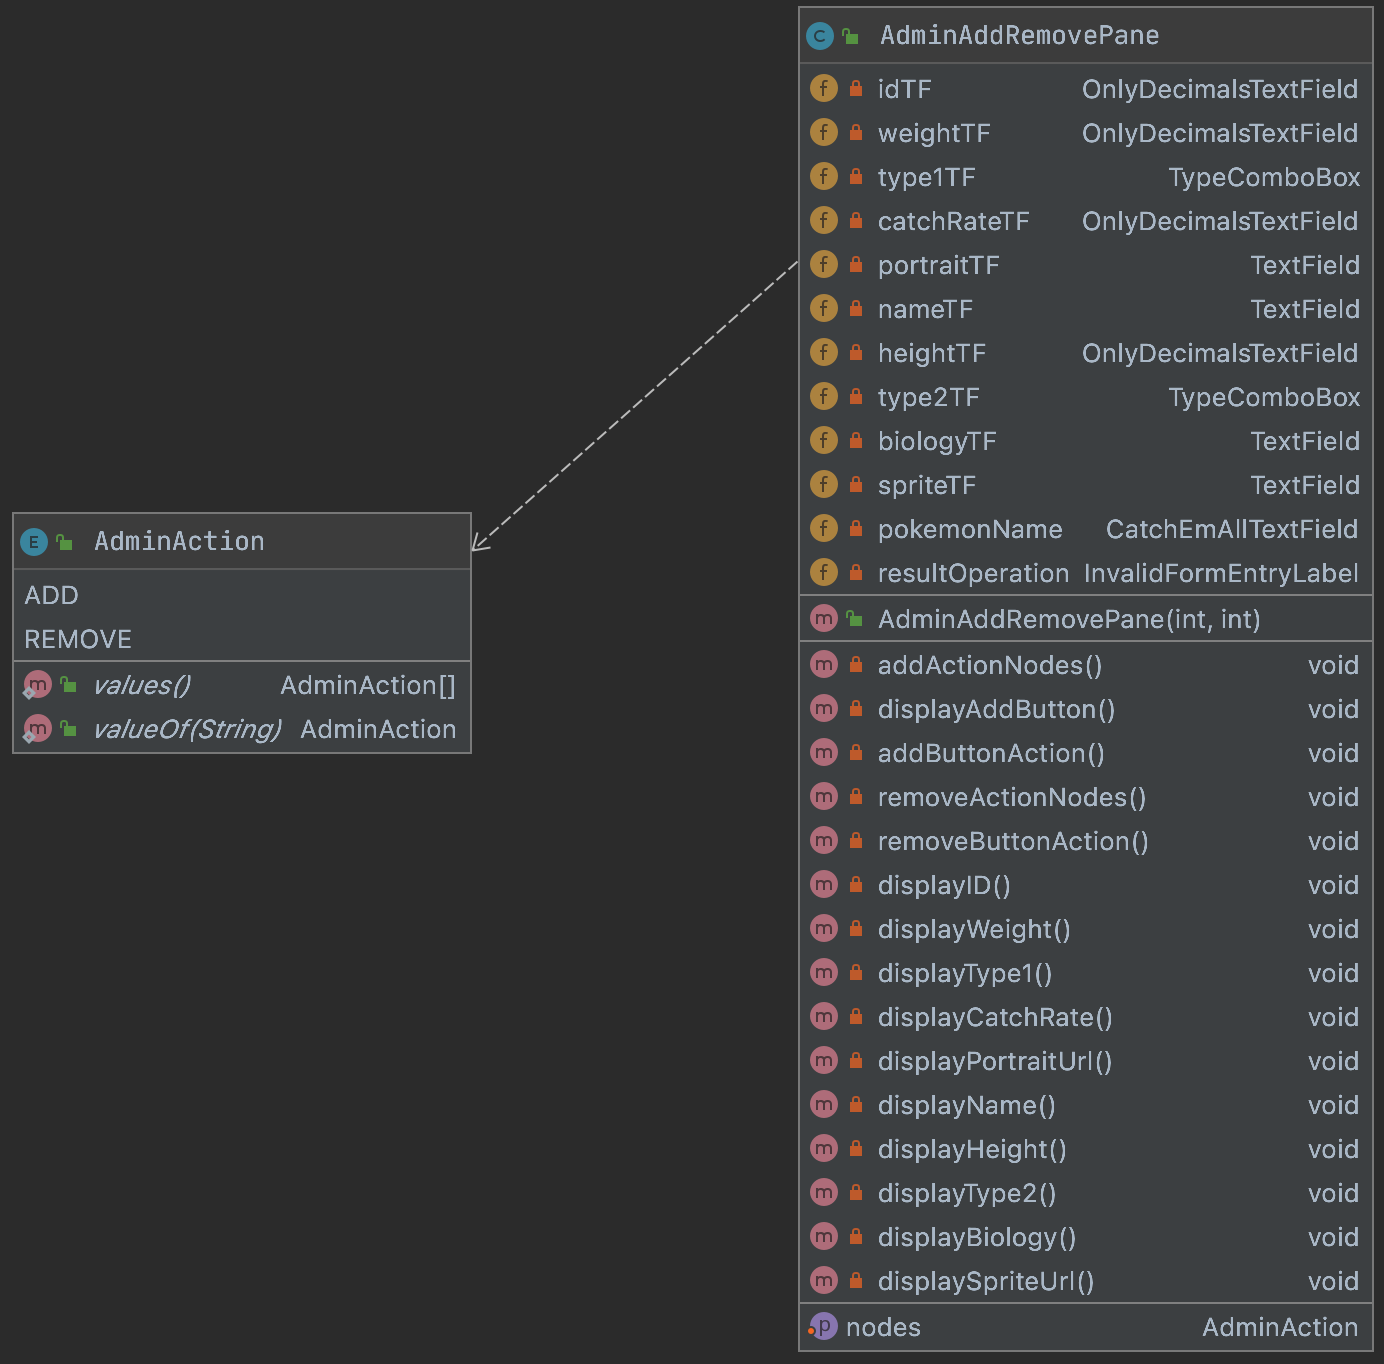
\includegraphics[width=0.7\textwidth]{img/javafx_panes_package3.png}
	\caption{javafxExtensions/panes/addRemove Package Class Structure}
\end{figure}
\begin{center}
	\begin{tabular}{| m{14em} | m{19em} |} 
		\hline
		\textbf{Class Name} & \textbf{Short Description} \\ [0.5ex] 
		\hline
		AdminAddRemovePane & Specific Pane for the ADD/REMOVE scene.\\ 
		\hline
		AdminAction & Contains the name of the action that an admin can do regarding the Pokemon management.\\ 
		\hline
	\end{tabular}
\end{center}


\subsubsection{Package Analysis: persistence}
The persistence package contains all the classes related to the communication with the databases. In the image below you can see how it is structured. The Factories classes are used as said before about the Ranking. 
\begin{figure}[H]
	\centering
	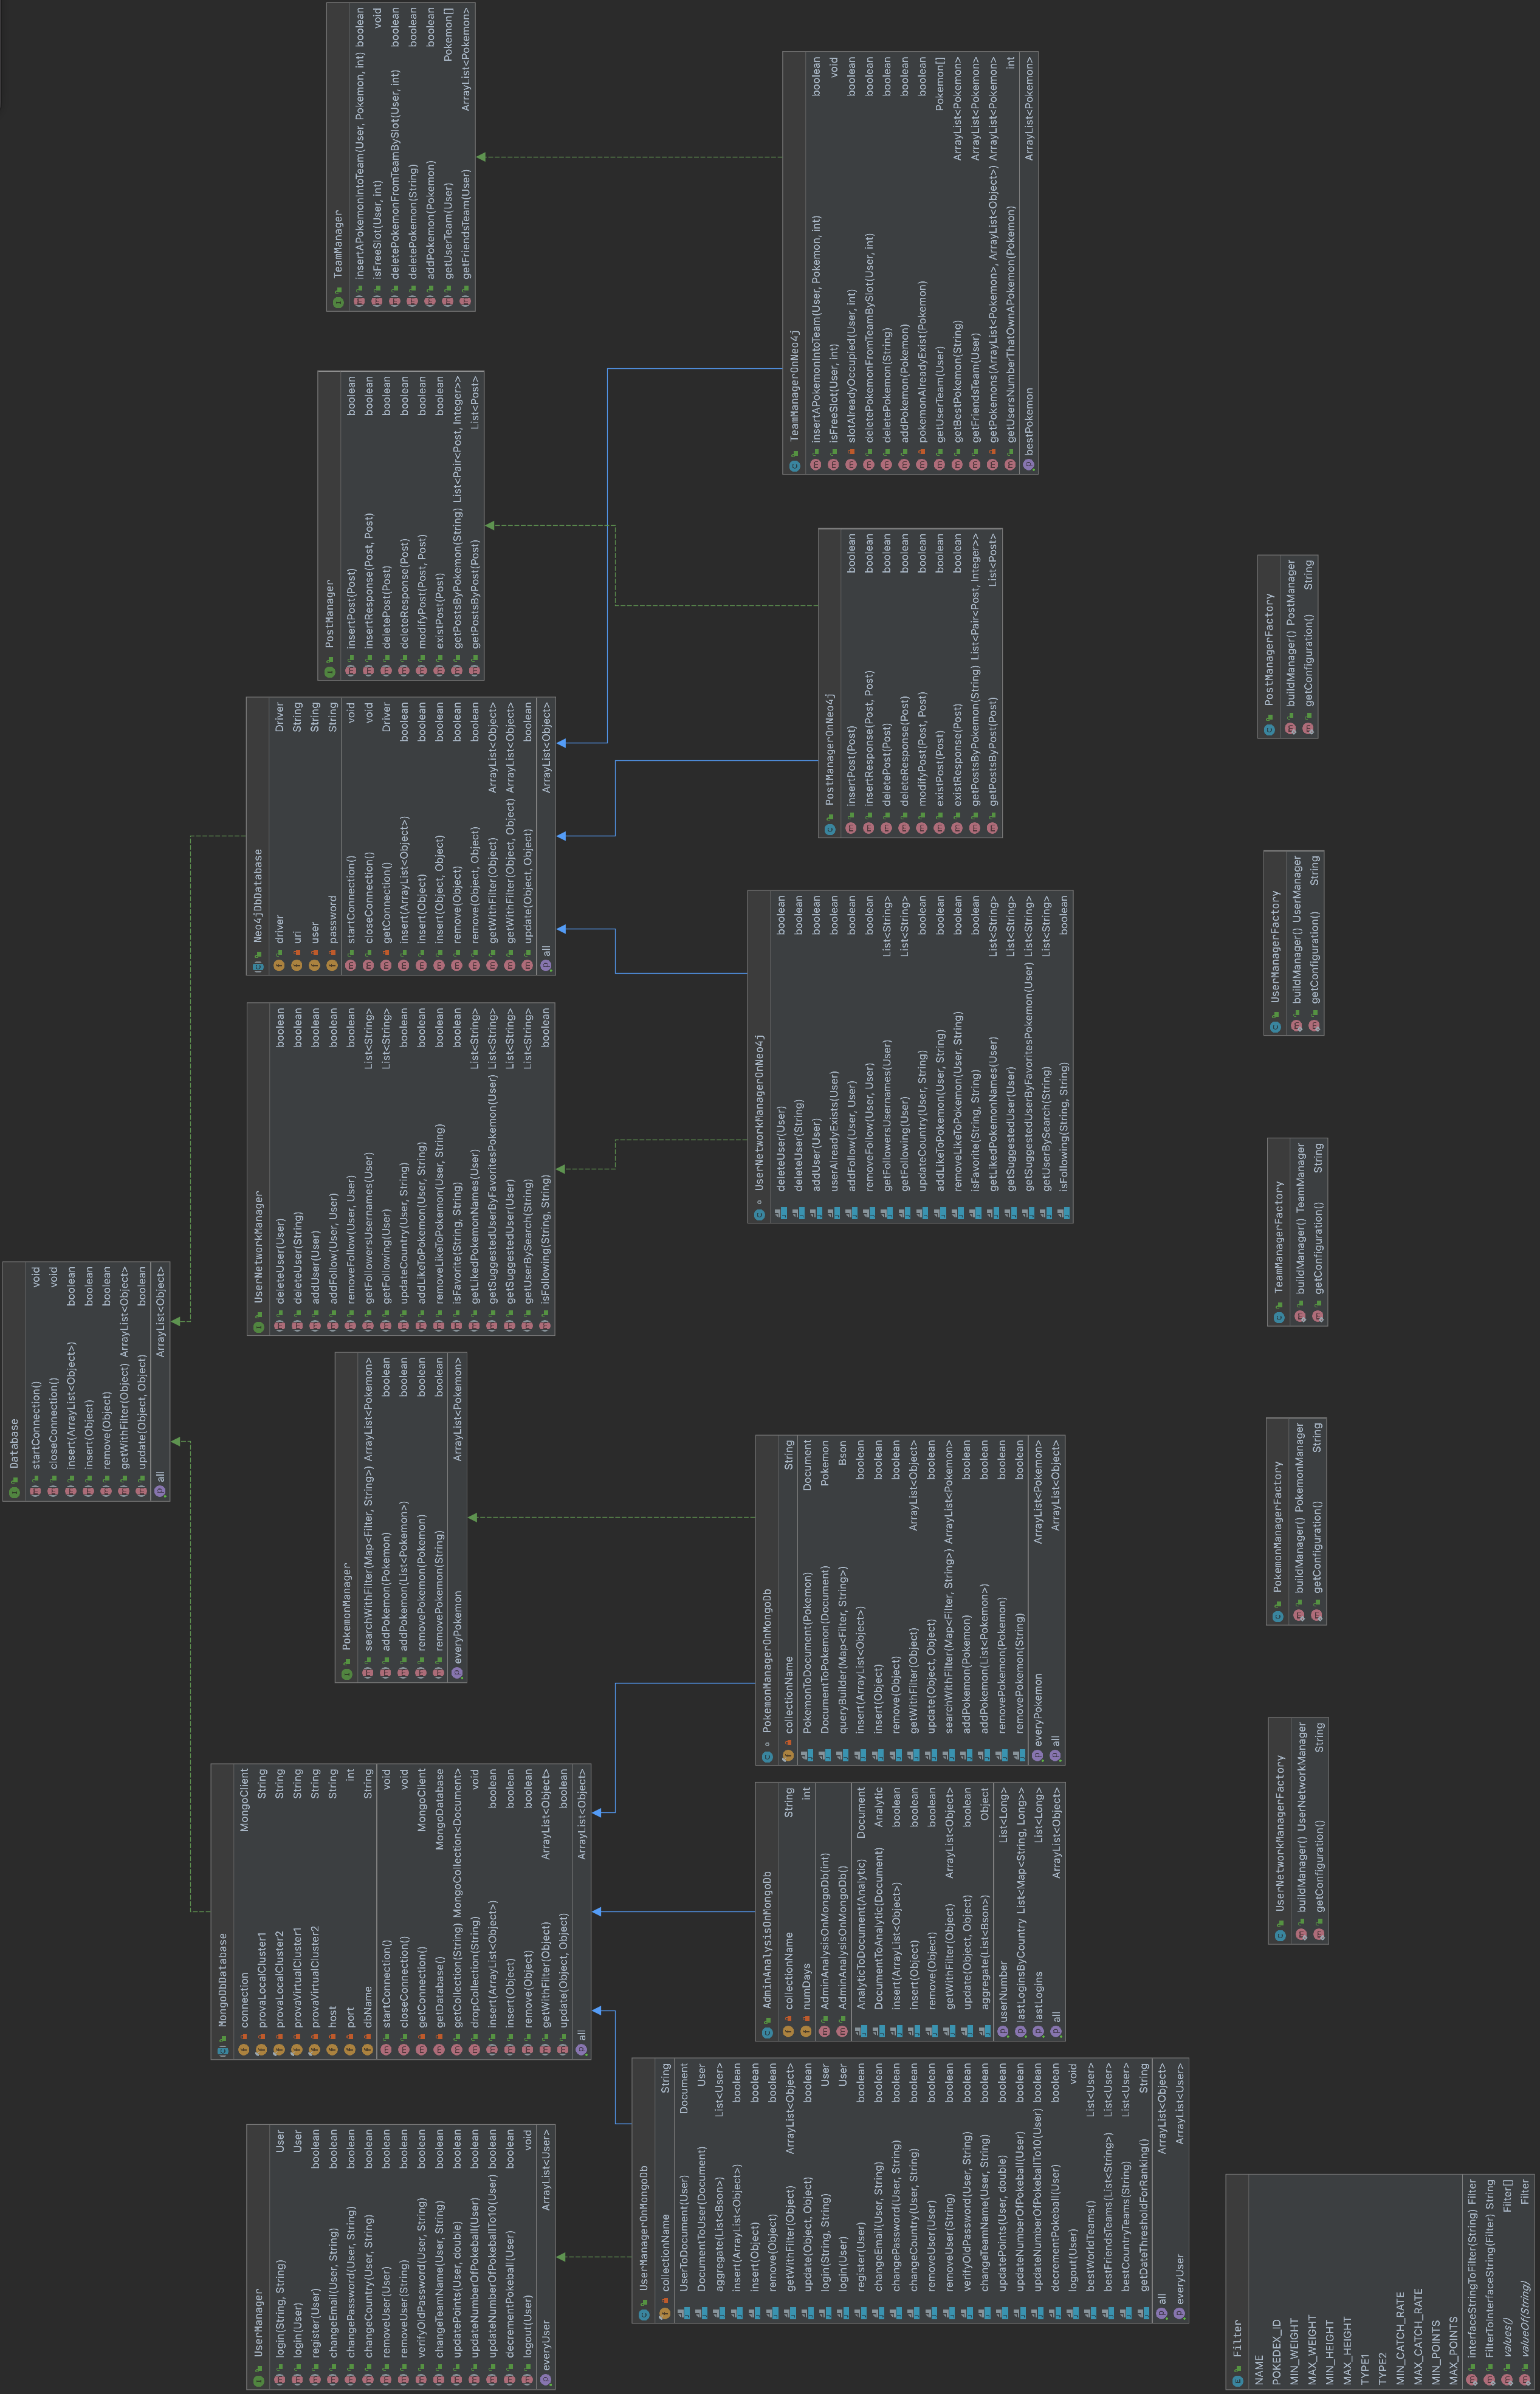
\includegraphics[width=0.9\textwidth]{img/persistence_package.png}
	\caption{persistence Package Class Structure}
\end{figure}

\begin{center}
	\begin{longtable}{| m{14em} | m{19em} |} 
		\hline
		\textbf{Class Name} & \textbf{Short Description} \\ [0.5ex] 
		\hline
		Database & Shared interface among Databases, defines remote connections and structures of basic CRUD operations\\ 
		\hline
		UserManager & Shared interface for the managing of users, defines the fundamental operations \\ 
		\hline
		PokemonManager & Shared interface for the managing of Pokemon, defines the fundamental operations \\ 
		\hline
		UserNetworkManager & Shared interface for the managing of Pokemon, defines the fundamental operations \\ 
		\hline
		PostManager & Shared interface for the managing of Post, defines the fundamental operations\\ 
		\hline
		MongoDbDatabase & Implementation of Database specific for MongoDB, to be extended with other classes.\\ 
		\hline
		UserManagerOnMongoDb & Extension of MongoDBDatabase, handles the user related queries in MongoDb\\ 
		\hline
		AdminAnalysisOnMongoDb & Extension of MongoDBDatabase, handles the admin related queries in MongoDb\\ 
		\hline
		PokemonManagerOnMongoDb & Extension of MongoDBDatabase, handles the Pokemon related queries in MongoDb\\ 
		\hline
		Neo4jDbDatabase & Implementation of Database specific for Neo4j, to be extended with other classes.\\ 
		\hline
		UserNetworkManagerOnNeo4j & Extension of Neo4jDbDatabase, handles the user related queries in Neo4j\\ 
		\hline
		PostManagerOnNeo4j & Extension of Neo4jDbDatabase, handles the post related queries in Neo4j\\
		\hline
		TeamManagerOnNeo4j & Extension of Neo4jDbDatabase, handles the Team related queries in Neo4j\\
		\hline
		Filter & Enum that contains the names of the filters used in the filter pane.\\
		\hline
		UserNetworkManagerFactory & Has a static method that returns a specific implementation of the interface UserNetworkManager\\
		\hline
		PokemonManagerFactory & Has a static method that returns a specific implementation of the interface PokemonManager\\
		\hline
		TeamManagerFactory & Has a static method that returns a specific implementation of the interface TeamManager.\\
		\hline
		UserManagerFactory & Has a static method that returns a specific implementation of the interface UserManager\\
		\hline
		PostManagerFactory & Has a static method that returns a specific implementation of the interface PostManager\\
		\hline
	\end{longtable}
\end{center}

\subsubsection{Package Analysis: security}
It contains the PasswordEncryptor class, we will discuss it in chapter 4.3.3


\subsubsection{Package Analysis: userInterface}
The userInterface package contains all the classes that are related to the creation of the GUI. The approach taken is a hierarchical one, in order to increase the modularity of the code.  
\begin{figure}[H]
	\centering
	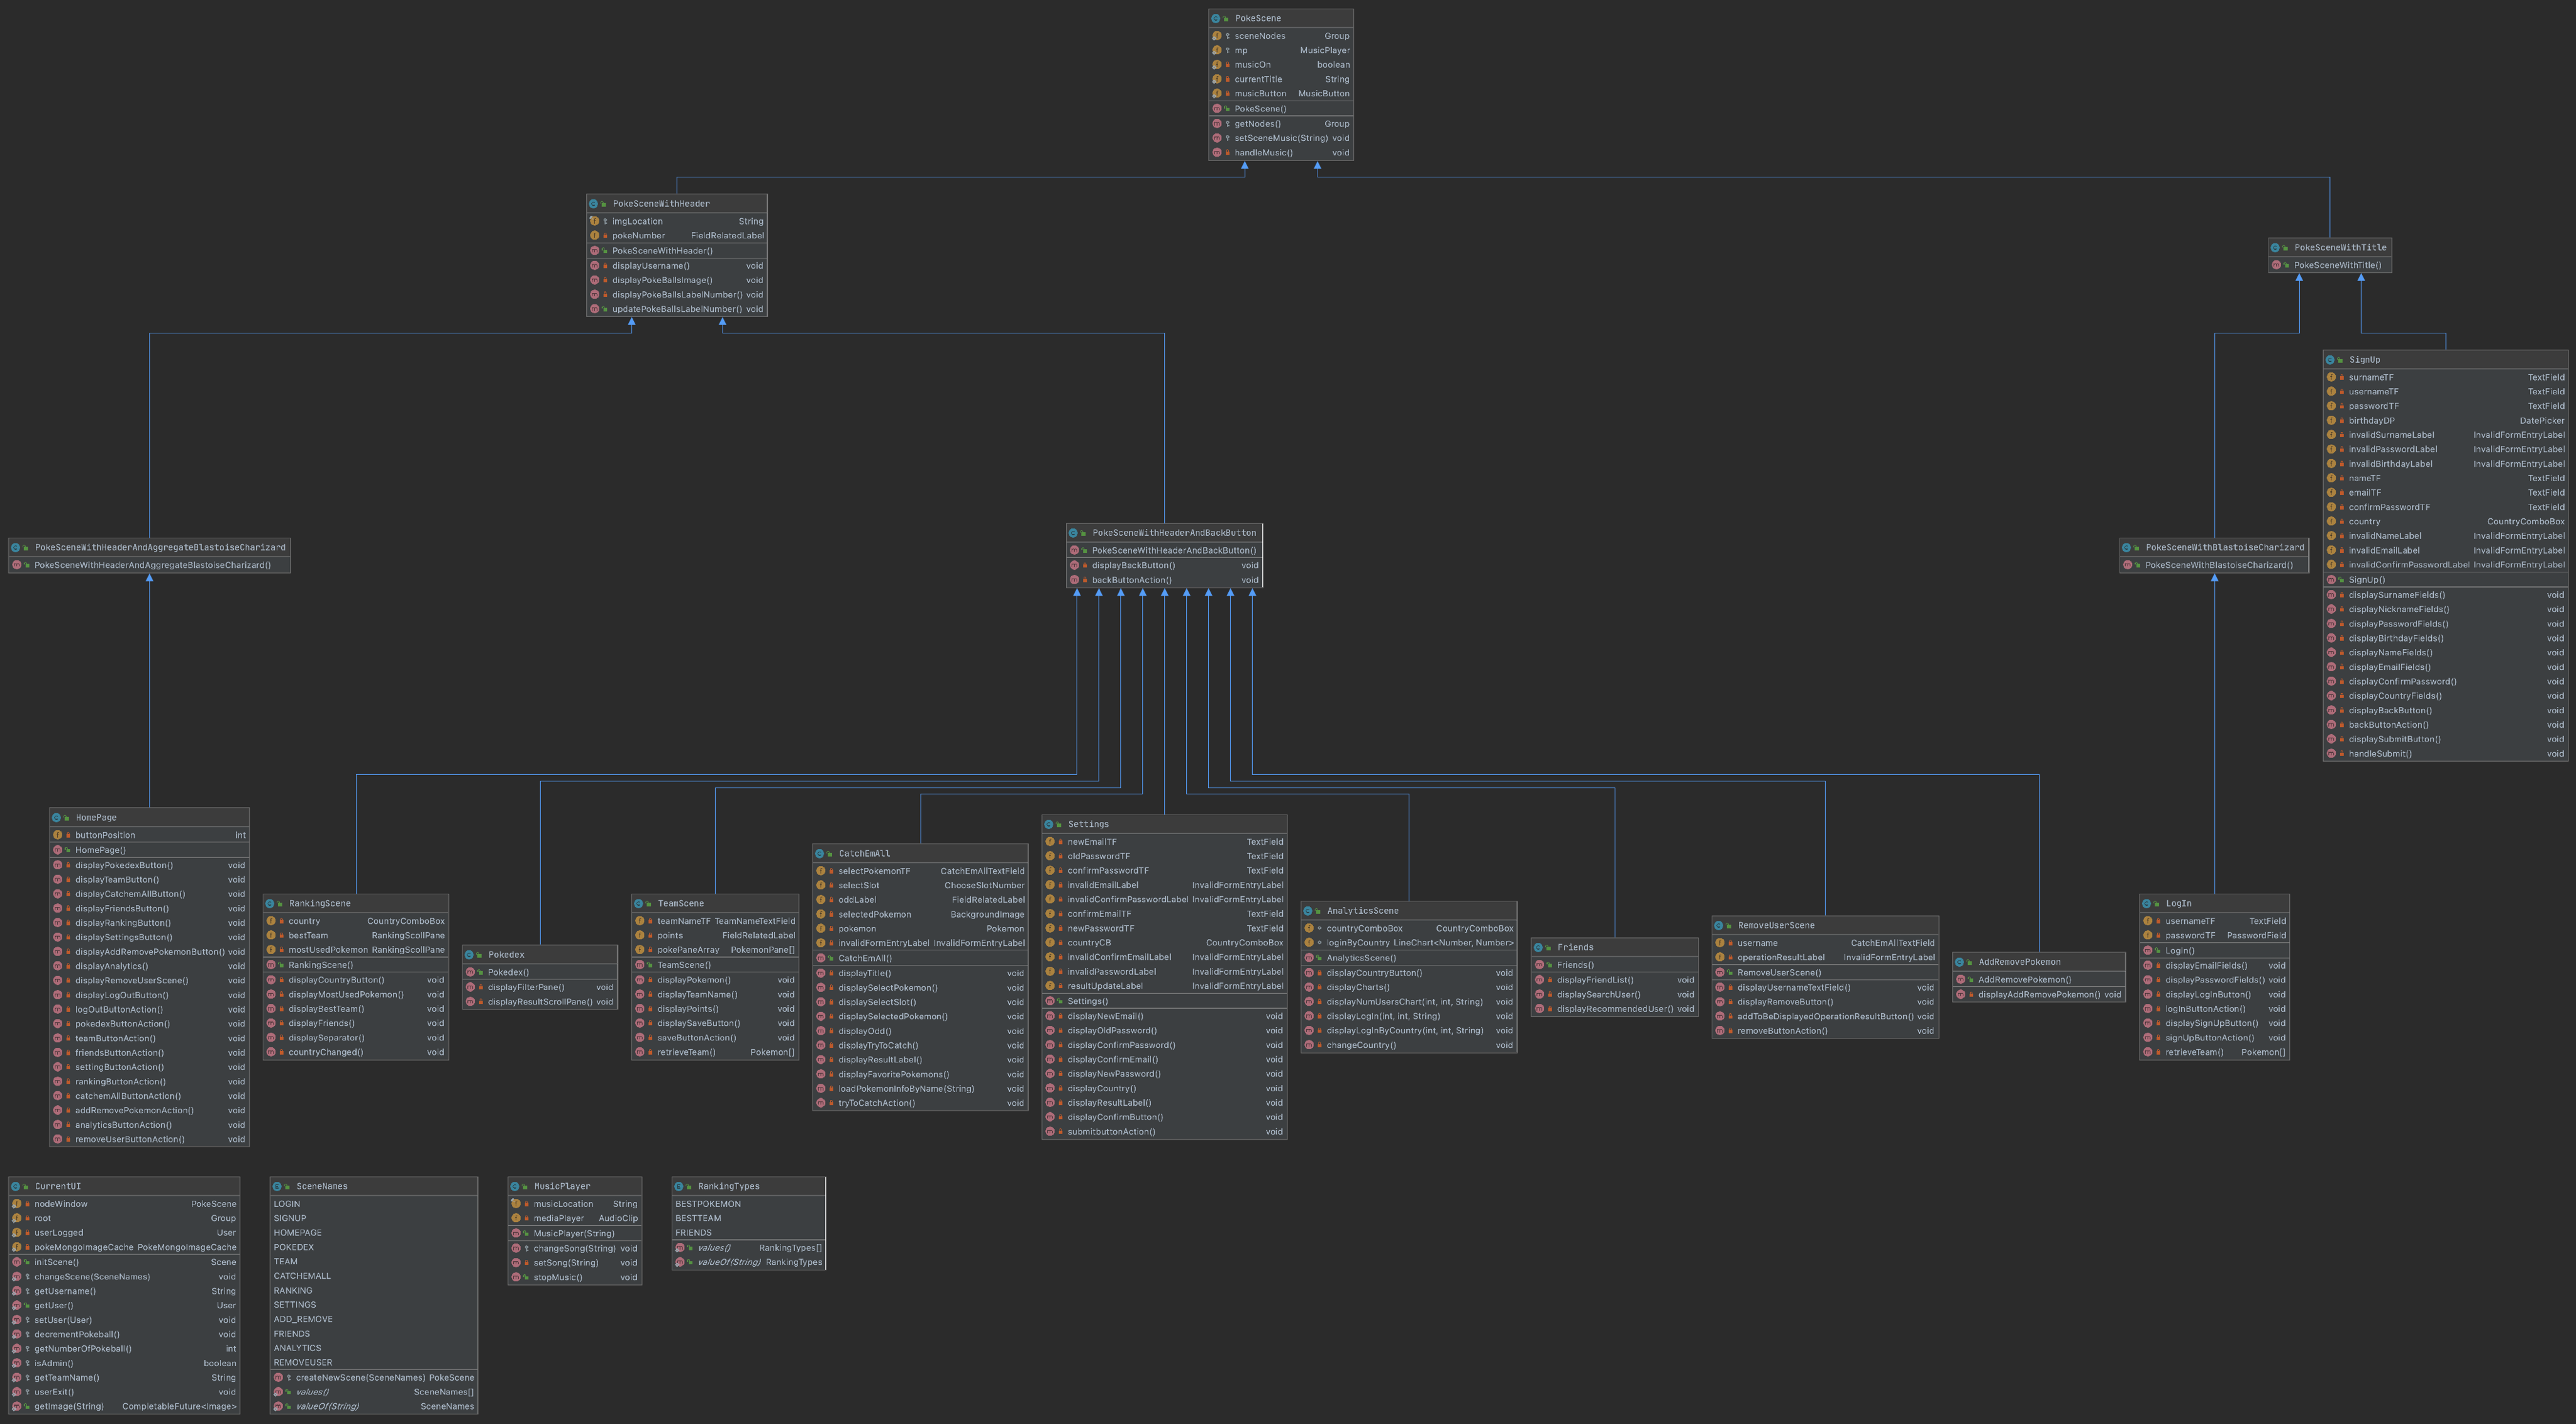
\includegraphics[width=\textwidth]{img/userInterface_package.png}
	\caption{userInterface Package Class Structure}
\end{figure}
\begin{center}
	\begin{longtable}{| m{14em} | m{19em} |} 
		\hline
		\textbf{Class Name} & \textbf{Short Description} \\ [0.5ex] 
		\hline
		PokeScene & General scene that contains the elements shared by every scene\\ 
		\hline
		PokeSceneWithHeader & General scene with only the Header in it (the header contains the username of the user logged and the number of pokemon)\\ 
		\hline
		PokeSceneWithTitle & General scene with only the title\\ 
		\hline
		SignUp & Sign up page\\ 
		\hline
		PokeSceneWithBlastoise Charizard & General scene that extends PokeSceneWithTitle and adds to the scene the image of Charizard and Blastoise\\ 
		\hline
		LogIn & The first scene the user will see at the opening of the application. As the name suggests the class displays the Nodes regarding the LogIn\\ 
		\hline
		PokeSceneWithHeaderAnd AggregateBlastoiseCharizard & General scene that combines the PokeSceneWithHeader and the PokeSceneWithBlastoiseCharizard\\ 
		\hline
		HomePage & As the name suggests the class displays the Nodes regarding the HomePage\\ 
		\hline
		PokeSceneWithHeaderAndBack Button & General scene that contains the Header and the Back Button\\ 
		\hline
		RankingScene & As the name suggests the class displays the Nodes regarding the Ranking\\ 
		\hline
		Pokedex & As the name suggests the class displays the Nodes regarding the Pokedex\\ 
		\hline
		TeamScene & As the name suggests the class displays the Nodes regarding the Team\\
		\hline
		CatchEmAll & As the name suggests the class displays the Nodes regarding the CatchEmAll page\\
		\hline
		Settings & As the name suggests the class displays the Nodes regarding the settings\\
		\hline
		AnalyticsScene & As the name suggests the class displays the Nodes regarding the admin analytics scene\\
		\hline
		Friends & As the name suggests the class displays the Nodes regarding the friend scene\\
		\hline
		RemoveUserScene & As the name suggests the class displays the Nodes regarding the remove user scene\\
		\hline
		AddRemovePokemon & As the name suggests the class displays the Nodes regarding the scene where the admin can add or remove a pokemon\\
		\hline
		SceneNames & Enum containing the different types of scene. Helps for the managing the changing in the scenes.\\
		\hline
		RankingTypes & Enum containing the different types of ranking\\
		\hline
		MusicPlayer & Handles the music.\\
		\hline
		CurrentUI & Handles the current UI. This is the bone of the entire package.\\
		\hline
	\end{longtable}
\end{center}
\subsubsection{Package Analysis: utils}
This package contains utility classes. 
\begin{figure}[H]
	\centering
	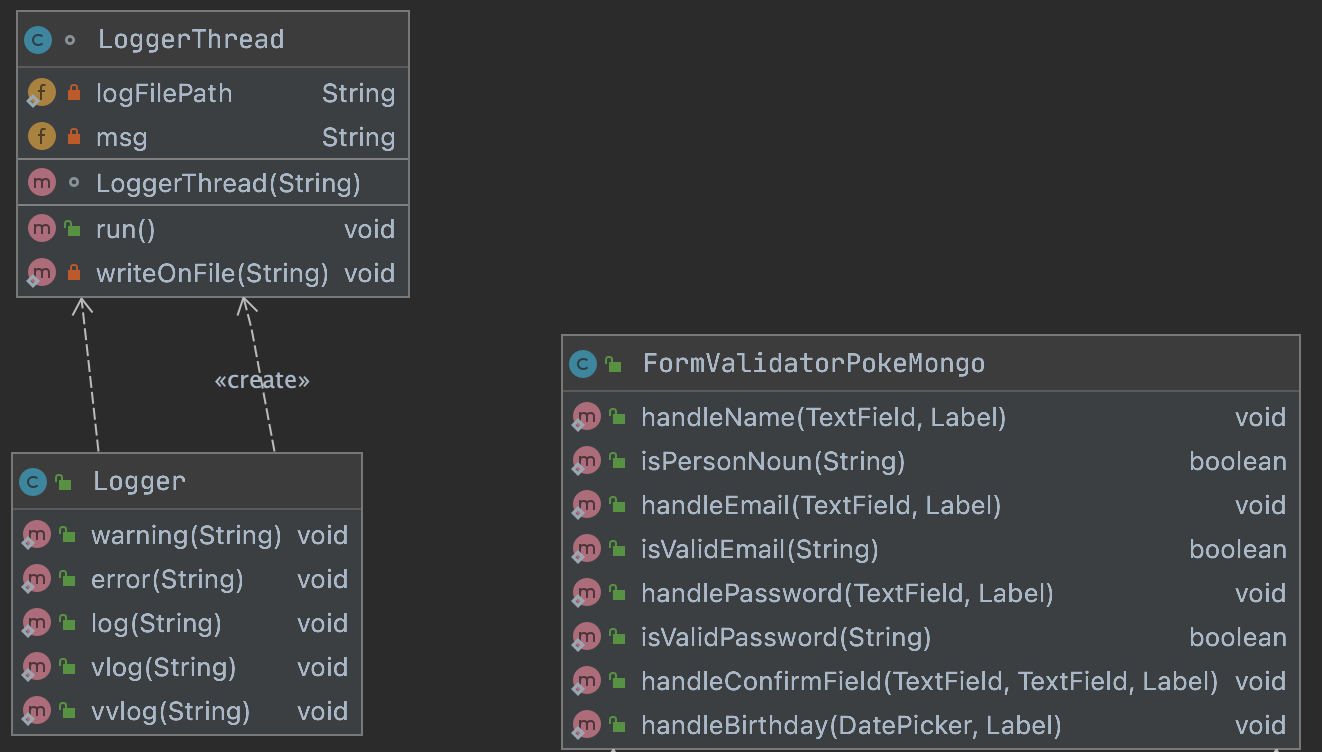
\includegraphics[width=0.7\textwidth]{img/utils_package.png}
	\caption{utils Package Class Structure}
\end{figure}
\begin{center}
	\begin{tabular}{| m{14em} | m{19em} |} 
		\hline
		\textbf{Class Name} & \textbf{Short Description} \\ [0.5ex] 
		\hline
		FormValidatorPokeMongo & Used for check if a field is well filled\\ 
		\hline
		LoggerThread & A thread that writes information about all the action taken by the code.\\ 
		\hline
	\end{tabular}
\end{center}

\subsubsection{Obfuscation}
Our package structure organization gave us the possibility to exploit code obfuscation. We use code obfuscation in the way to hide how the connection of the database is done. To do that we limited some classes to have only a package scope and, to interact with them, we use the Manager classes presented before.

\subsection{APIs and SPIs}

\subsection{Main tools}
\subsubsection{GSON}
\subsubsection{Caching mechanism and multimedia management}
\subsubsection{Password Encryptor}
\subsubsection{Logger}

\subsection{Analytics queries}
\subsubsection{User Rankings}
\subsubsection{Pokémon Rankings}
\subsubsection{Usage Statistics}
\subsubsection{Dynamic Catch Rate}


\subsection{Business logic}
\subsubsection{Points computing}
\subsubsection{Dynamic Catch Rate Computing}


